%-----------------------------------------------------------------------
\begin{figure*}[!t]
  \begin{center}
  \scalebox{0.95}{
  \begin{tabular}{cc}
    \subfigure[JMeter (LOC)]{ 
      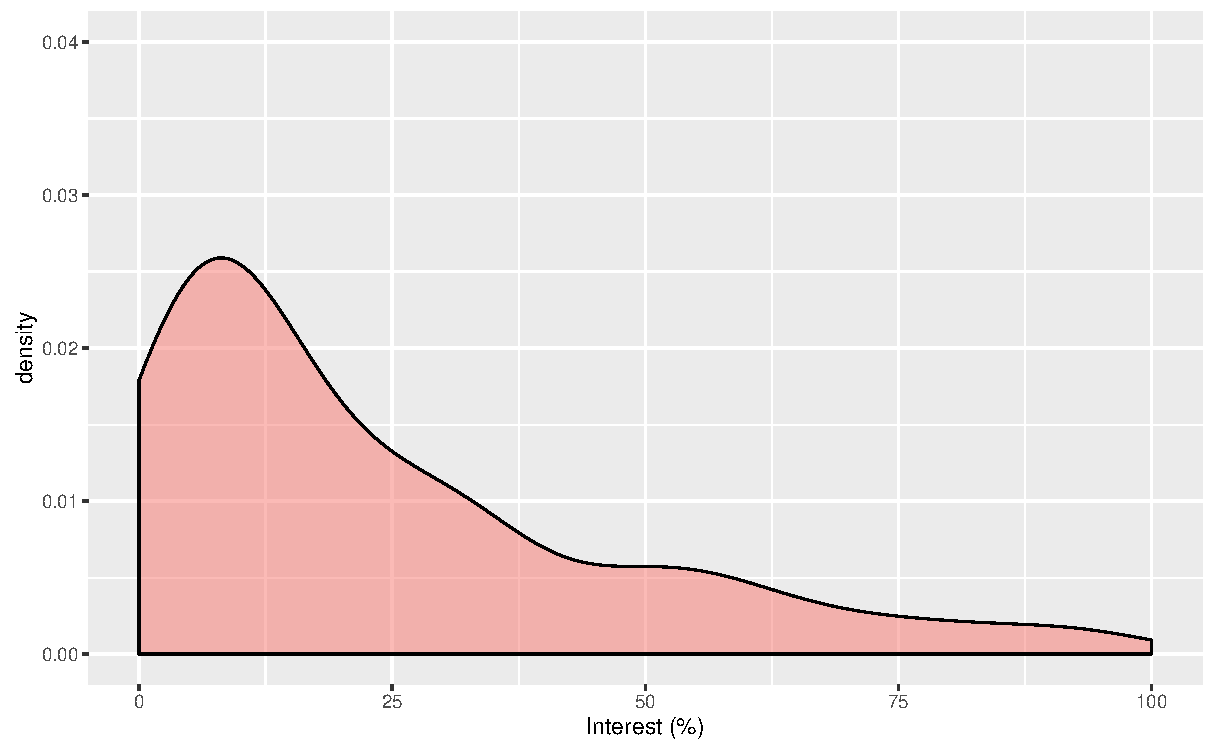
\includegraphics[width=.45\textwidth]{figures/rq1-jmeter}
    }
    \subfigure[JMeter (Fan-In)]{ 
      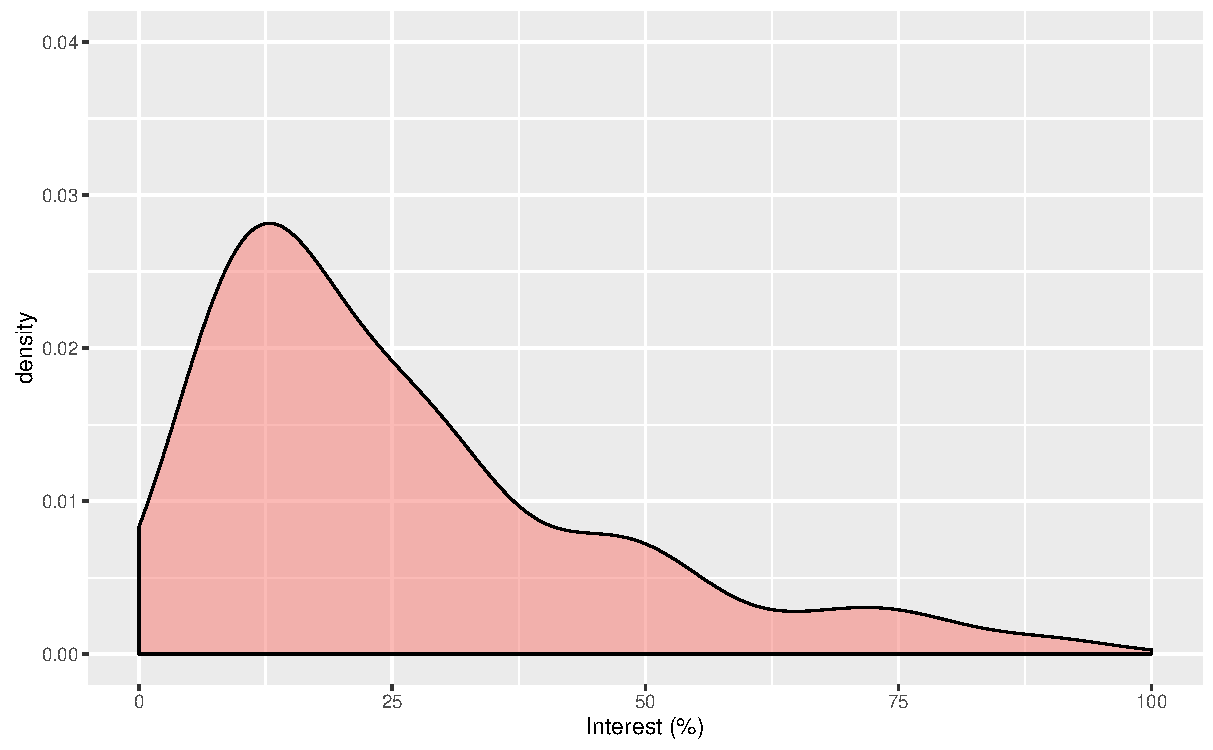
\includegraphics[width=.45\textwidth]{figures/rq1-jmeter-fanin}
    }
  \end{tabular}
  }

  \caption{The results of distribution of interest.}
  \label{fig:dist}
  \end{center}
\end{figure*}
%-----------------------------------------------------------------------


\section{Initial Case Study} \label{sec:results}
\smallsection{Motivation}
To alleviate the impact of technical debt, there are several previous studies on understanding SATD (e.g., the detection of technical debt~\cite{Potdar2014ICSME,Zazworka2013EASE} and the impact of SATD on software quality~\cite{Wehaibi2016SANER}).
However, there are few empirical studies that quantify interest of SATD.
Therefore, we would like to know how we can understand interest using our method explained in Section \ref{sub:approach}

\smallsection{Datasets}
To conduct our initial case study, we use data from one open source software projects (Apache Jmeter). The dataset was used in previous studies~\cite{Maldonado2015MTD,Potdar2014ICSME}. The project uses Git as a version control system. Table \ref{tab:project} shows the statistics of the project we use in our experiments. 

\begin{table}[tb]
  \caption{Project details}
  \label{tab:project}
  \centering

  \begin{tabular}{l|rrrp{1.0cm}p{1.0cm}}
  \hline
    Project & Release & \# of classes & SLOC & \# of comments & \# of contributors \\
  \hline
    JMeter & xxx &   x  &    x  &        x  &    x   \\
  \hline
  \end{tabular}
\end{table}

%\todo{How do we choose projects we analyze? i.e., why do we use Ant and Jmeter and do not use ArgoUML, Columba and JFreeChart? and why do we add jRuby?}


\smallsection{Approach}
%\para{We calculate the interest.}
To calculate interest of SATD, we follow the approach we explained in Section \ref{sec:setup}.
We show the number of SATD, the percentage of the technical debt that has positive interest, and the distribution of interest for technical debt of positive rate.

\smallsection{Results}
We find that there are high correlations between LOC and the other product metrics except Fan-In. 
From the highly correlated metrics, we choose LOC as metrics to calculate interest, similar to previous work that considers effort in the domain of defect prediction~\cite{Kamei2010ICSM,Kamei2013TSE}. We assume that developers spend more effort to check larger methods before modifying the methods. Eventually, we show our results using two product metrics (i.e., LOC and Fan-In).

Table \ref{tab:percentage} shows the number of SATD and the percentage of the technical debt that has positive interest in all technical debt. The table shows that 32.6\%-44.2\% of technical debt has a positve rate in terms of LOC and 30.9\%-42.2\% of technical debt has it in terms of Fan-In. 
There is not large difference of the positive rates between LOC and Fan-In. 
% The positive rate of LOC in ANT is 38.0% 

Figure \ref{fig:dist} and Table \ref{tab:statistic} show that the distribution of interest for the technical debt of positive rate. The distribution in LOC plots are left-skewed (around 0 to 10). We can also find that some of positive interest are over 100, which means the value of metric relatively increases by 100\%.
This findings suggest that we have the technical debt that we preferentially allocate development effort.


\begin{table}[tb]
  \caption{The percentage of SATD that has positive interest}
  \label{tab:percentage}
  \centering

  \begin{tabular}{c|r|rrr}
  \hline
        & Positive Rate & All & Positive & Negative \\
  \hline
   LOC  & 44.2\% & 181 &  80  &  25 \\
Fan-In  & 42.2\% & 161 &  68  &  13 \\
  \hline
  \end{tabular}
\end{table}

\begin{table}[tb]
  \caption{Statistics}
  \label{tab:statistic}
  \centering

  \begin{tabular}{c|rrrrr}
  \hline
        & Min. & 1st Qu. & Median & 3rd Qu. & Max. \\
  \hline
   LOC  & 1.6 &   6.9 &  18.0  &   50.0 & 6667.0 \\
Fan-In  & 5.6 &  12.4 &  25.0  &   50.0 &  900.0 \\
  \hline
  \end{tabular}
\end{table}

\conclusionbox{
44.2\% of technical debt has a positive rate in terms of LOC and 42.2\% of technical debt has it in terms of Fan-In.}


%\para{Put additional analysis when considering time period.}

%\para{Put additional analysis when considering other metrics (fan-in).}

%\para{Put the analysis for showing the method that includes more than one technical debt in one version.}